\chapter{Bridge Pattern}

\section{Định nghĩa}
Bridge Pattern là một trong những Pattern thuộc nhóm cấu trúc (Structural Pattern). Ý tưởng của nó là tách phần trừu tượng (abstraction) ra khỏi tính hiện thực (implementation) của nó. Từ đó có thể dễ dàng chỉnh sửa hoặc thay thế mà không làm ảnh hưởng đến những nơi có sử dụng lớp ban đầu. Điều đó có nghĩa là, ban đầu chúng ta thiết kế một class với rất nhiều tiến trình, bây giờ chúng ta không muốn để những tiến trình đó trong class đó nữa. Vì thế, chúng ta sẽ tạo ra một class khác và di chuyển các tiến trình đó qua class mới. Khi đó, trong lớp cũ sẽ giữ một đối tượng thuộc về lớp mới, và đối tượng này sẽ chịu trách nhiệm xử lý thay cho lớp ban đầu.

\section{Mục đích sử dụng}
\begin{itemize}
\item Tách ràng buộc giữa Abstraction (phần trìu tượng) và Implementation (phần thực thi) để có thể dễ dàng mở rộng độc lập nhau. Thay vì liên hệ với nhau bằng quan hệ kế thừa, hai thành phần này liên hệ với nhau thông qua quan hệ “chứa trong” (object composition).
\item Sử dụng khi cả Abstraction và Implementation của chúng nên được mở rộng bằng subclass.
\item Sử dụng ở những nơi mà những thay đổi được thực hiện trong implement không ảnh hưởng đến phía client.
\end{itemize}

\section{Mô hình cấu trúc}
\begin{center}
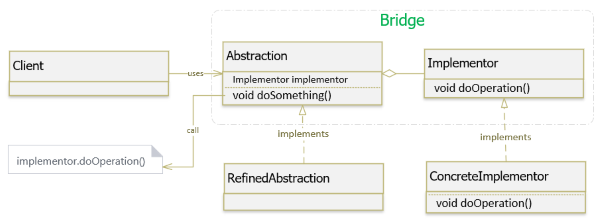
\includegraphics{GALLEYS/images/chapter8/diagram}
\end{center}
Các thành phần:
\begin{itemize}
\item Client: đại diện cho khách hàng sử dụng các chức năng thông qua Abstraction.
\item Abstraction: định ra một abstract interface quản lý việc tham chiếu đến đối tượng hiện thực cụ thể (Implementor).
\item Refined Abstraction (AbstractionImpl): hiện thực (implement) các phương thức đã được định ra trong Abstraction bằng cách sử dụng một tham chiếu đến một đối tượng của Implementer.
\item Implementor: định ra các interface cho các lớp hiện thực. Thông thường nó là interface định ra các tác vụ nào đó của Abstraction.
\item ConcreteImplementor: hiện thực Implementor interface.
\end{itemize}
Để có thể hiểu rõ hơn, chúng ta xét ví dụ cụ thể sau: Một hệ thống ngân hàng cung cấp các loại tài khoản khác nhau cho khách hàng, chẳng hạn: Checking account và Saving account. Chúng ta có sơ đồ như sau:
\begin{center}
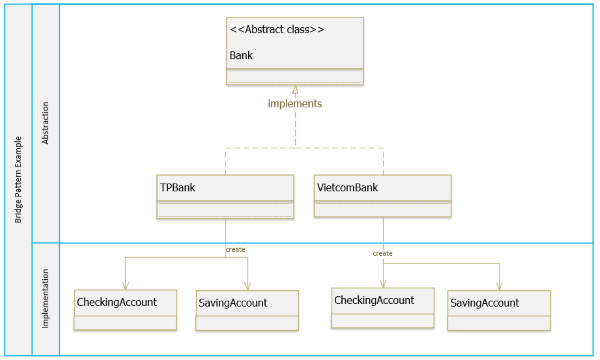
\includegraphics{GALLEYS/images/chapter8/examplepic1}
\end{center}
Với cách thiết kế như vậy, khi hệ thống cần cung cấp thêm một loại tài khoản khác, chúng ta phải tạo class mới cho tất cả các ngân hàng, số lượng class tăng lên rất nhiều. Bây giờ, chúng ta sẽ sử dụng Bridge Pattern để tái cấu trúc lại hệ thống trên như sau:
\begin{center}
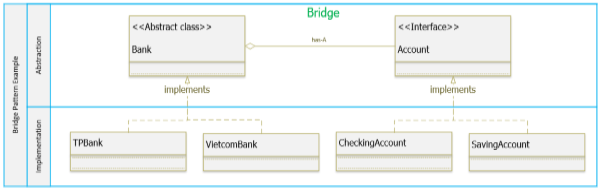
\includegraphics{GALLEYS/images/chapter8/examplepic2}
\end{center}
Với cấu trúc mới như vậy, khi có thêm một loại tài khoản mới, chúng ta đơn giản chỉ việc thêm vào một implement mới cho Account, các thành phần khác của Bank không bị ảnh hưởng. Hoặc cần thêm một ngân hàng mới, chẳng hạn VietinBank chúng ta chỉ cần thêm implement mới cho Bank, các thành phần khác cũng không bị ảnh hưởng và số lượng class chỉ tăng lên 1. Code cho chương trên như sau:\\
\newpage
\textbf{Account.java}
\begin{center}
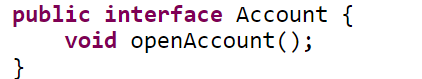
\includegraphics{GALLEYS/images/chapter8/code1}
\end{center}
\textbf{CheckingAccount.java}
\begin{center}
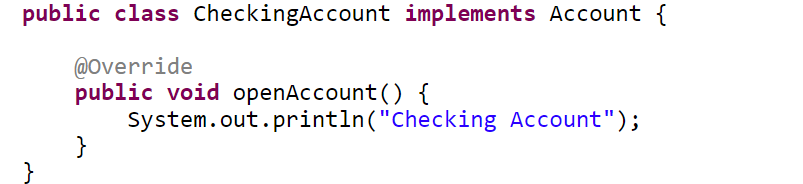
\includegraphics{GALLEYS/images/chapter8/code2}
\end{center}
\textbf{SavingAccount.java}
\begin{center}
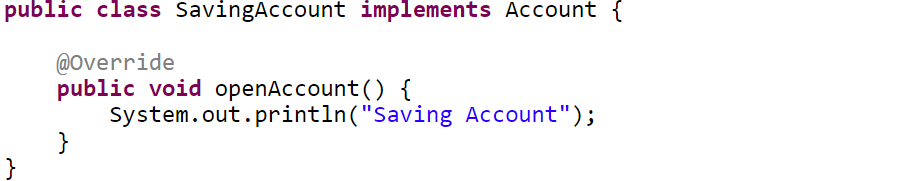
\includegraphics{GALLEYS/images/chapter8/code3}
\end{center}
\newpage
\textbf{Bank.java}
\begin{center}
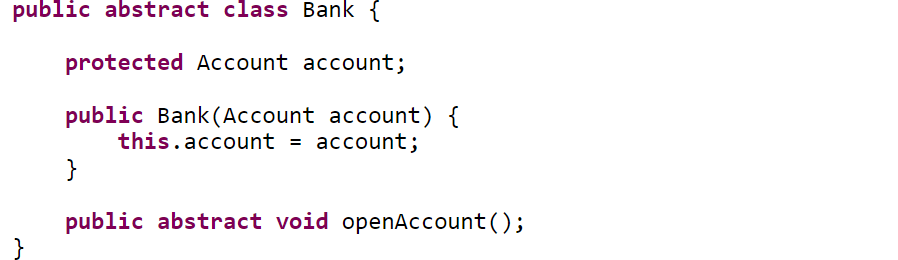
\includegraphics{GALLEYS/images/chapter8/code4}
\end{center}
\textbf{VietcomBank.java}
\begin{center}
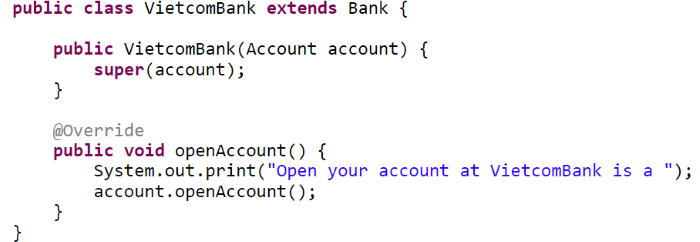
\includegraphics{GALLEYS/images/chapter8/code5}
\end{center}
\newpage
\textbf{TPBank.java}
\begin{center}
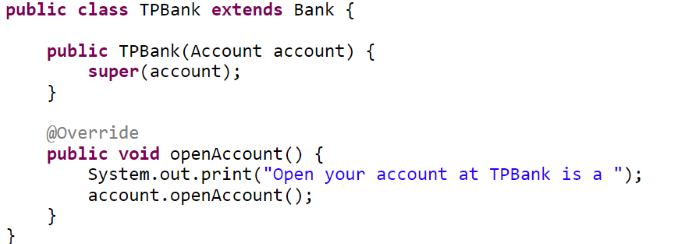
\includegraphics{GALLEYS/images/chapter8/code6}
\end{center}
\textbf{Client.java}
\begin{center}
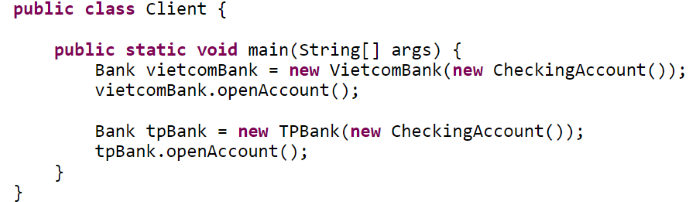
\includegraphics{GALLEYS/images/chapter8/code7}
\end{center}
\textbf{Và cuối cùng là output của chương trình:}\\
\textbf{Open your account at VietcomBank is a Checking Account}\\
\textbf{Open your account at TPBank is a Checking Account}

\section{Bridge Pattern trong thực tế}
Hầu như trong mọi ứng dụng chúng ta cần lưu trữ dữ liệu. Giả sử chúng ta cần lưu trữ trong 2 cơ chế lưu trữ khác nhau là tệp và cơ sở dữ liệu. Ngoài ra, trước khi chúng ta lưu trữ, chúng ta phải xử lý đối tượng [xác thực, thiết lập một vài dữ liệu, v.v.]. Thông thường, chúng ta sử dụng các lớp riêng biệt để thực hiện các quy trình này như dưới đây:
\begin{multicols}{2}
	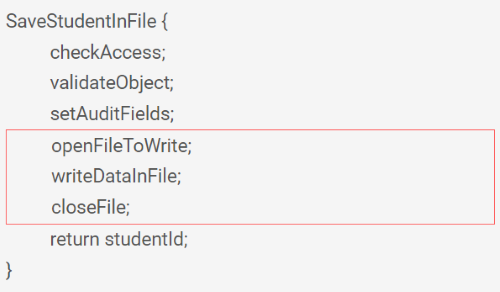
\includegraphics[width=1\columnwidth]{GALLEYS/images/chapter8/app1}
	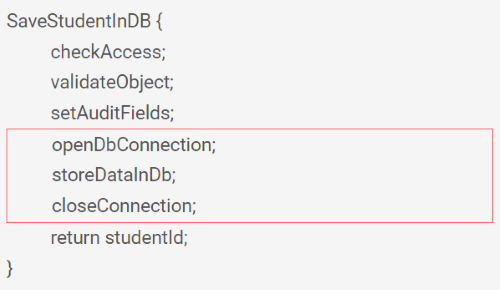
\includegraphics[width=1\columnwidth]{GALLEYS/images/chapter8/app2}
\end{multicols}
Chúng ta có code để lưu trữ đối tượng Student vào tệp và cơ sở dữ liệu. Đây là một kịch bản phổ biến. Bây giờ, hãy giả sử rằng chúng ta cần thêm code để làm điều tương tự cho đối tượng khóa học (course). Sau đó, chúng ta sẽ cần hai lớp nữa như SaveCourseInFile và SaveCourseInDB.

Ngoài ra, nếu chúng ta cần thêm hệ thống lưu trữ mới như cơ sở dữ liệu hoặc yêu cầu mạng (network call) khác thì chúng ta sẽ phải tạo lớp mới cho mỗi loại. Giống như ví dụ của chúng ta là lớp Student và lớp Course. Điều này sẽ tiếp tục tăng đối với từng lớp và loại lưu trữ mới. Bridge Pattern đơn giản hóa tình huống trên bằng cách giúp chúng ta viết code có thể tái sử dụng.